\chapter*{Обзор литературы}                         % Заголовок
\addcontentsline{toc}{chapter}{Обзор литературы}    % Добавляем его в оглавление

Возникновение теории биологической эволюции берет свое начало в 18 - ом веке. Одним из первых, кто попытался выяснить как протекает процесс эволюции был выдающийся французский ученый - естествоиспытатель, Жан Батист Ламарк. Именно он в 1802 году впервые ввел термин ``биология''\,. В своем труде, ``Философия зоологии''\, \cite{Lamark} (1809), Ламарк утверждал, что движущими силами эволюции являются изменения окружающей среды.

В дальнейшем эта теория была развита Чарльзом Дарвином, английским натуралистом и путешественником, человеком, который вошел в историю как основоположник современной теории эволюции. Дарвином было проделано множество различных экспериментов, результатом которых стал его знаменитый труд --- ``Происхождение видов путем естественного отбора''\, \cite{Darwin} (1859). В этой работе были изложены три основных дарвинских принципа эволюции: наследственность, изменчивость и естественный отбор.  

\begin{figure}[ht]
\centerfloat{
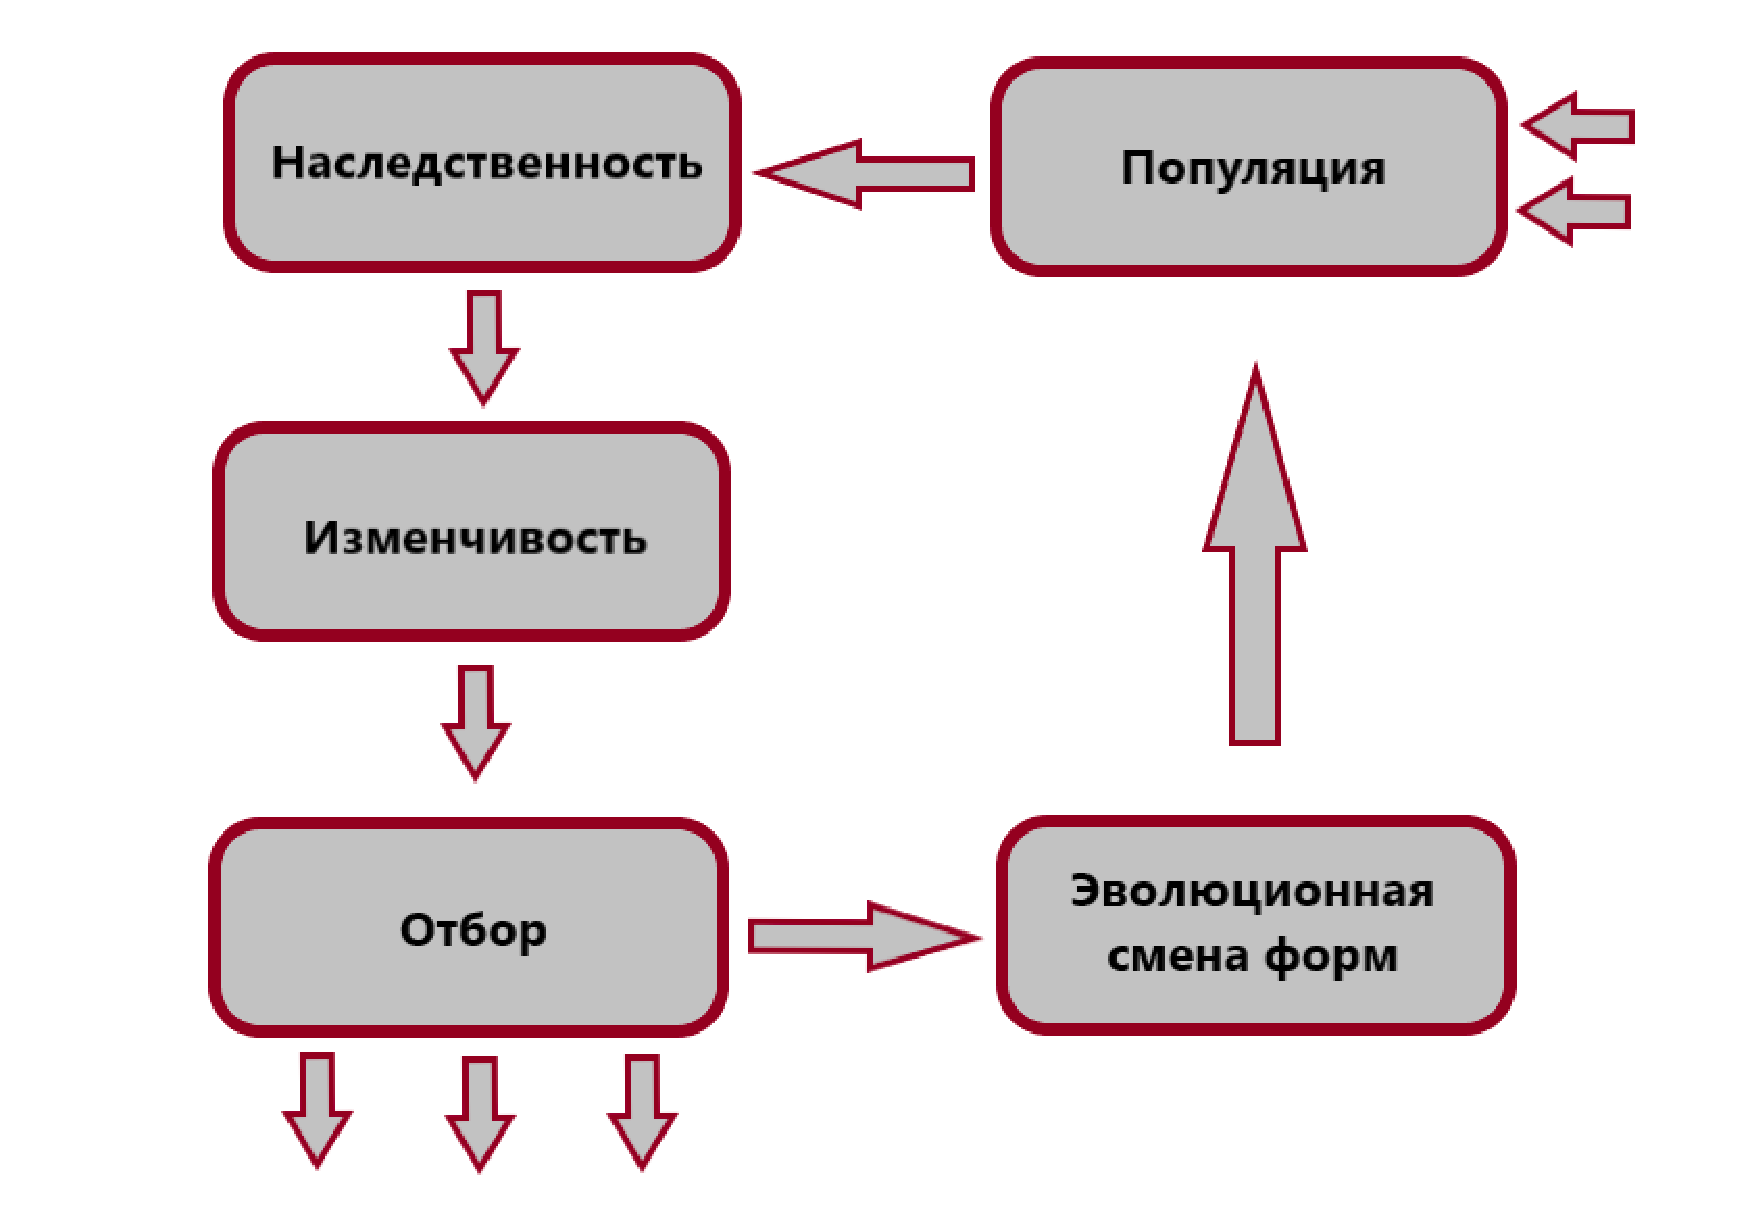
\includegraphics[width = 0.9\linewidth]{darwin.eps}
}
\caption{Схема эволюции Ч. Дарвина.}
\label{lr_fig1}
\end{figure}

Согласно Дарвину, живые организмы в течение всей своей жизни претерпевают различные мутации, которые могут быть обусловлены изменениями окружающей среды или возникновением конкуренции между соседствующими организмами. Это приводит к исчезновению старых признаков и появлению новых, более выгодных, которые затем наследуют потомки. Схематически принципы Дарвина можно изобразить так, как это показано на рис. \ref{lr_fig1}.

Из личных записей Дарвина известно, что он читал работу Томаса Мальтуса --- автора теории ``народонаселения''\, или, как ее еще называют, теории ``Мальтузианства''\, \cite{Malthus}, опубликованную в 1978 году и был впечатлен полученными результатами. Основная идея теории Мальтуса заключалась в том, что в условиях неограниченности ресурсов, численность населения растет по закону геометрической прогрессии, в то время как скорость производства пищевых продуктов --- линейна. Результатом такого процесса является состояние, которое принято называть ``Мальтузианской ловушкой''\, (рис. \ref{lr_fig2}), то есть ситуацией при которой численность населения превосходит количество произведенных продуктов питания. 

Но Дарвин не был знаком с работой бельгийского математика Пьера Ферхюльста \cite{Verhlust} (1838). Ферхюльст модифицировал модель Мальтуса, добавив туда дополнительный член, характеризующий предельную величину численности популяции. Впоследствии его закон получил название логистического уравнения.

\begin{figure}[ht]
\centerfloat{
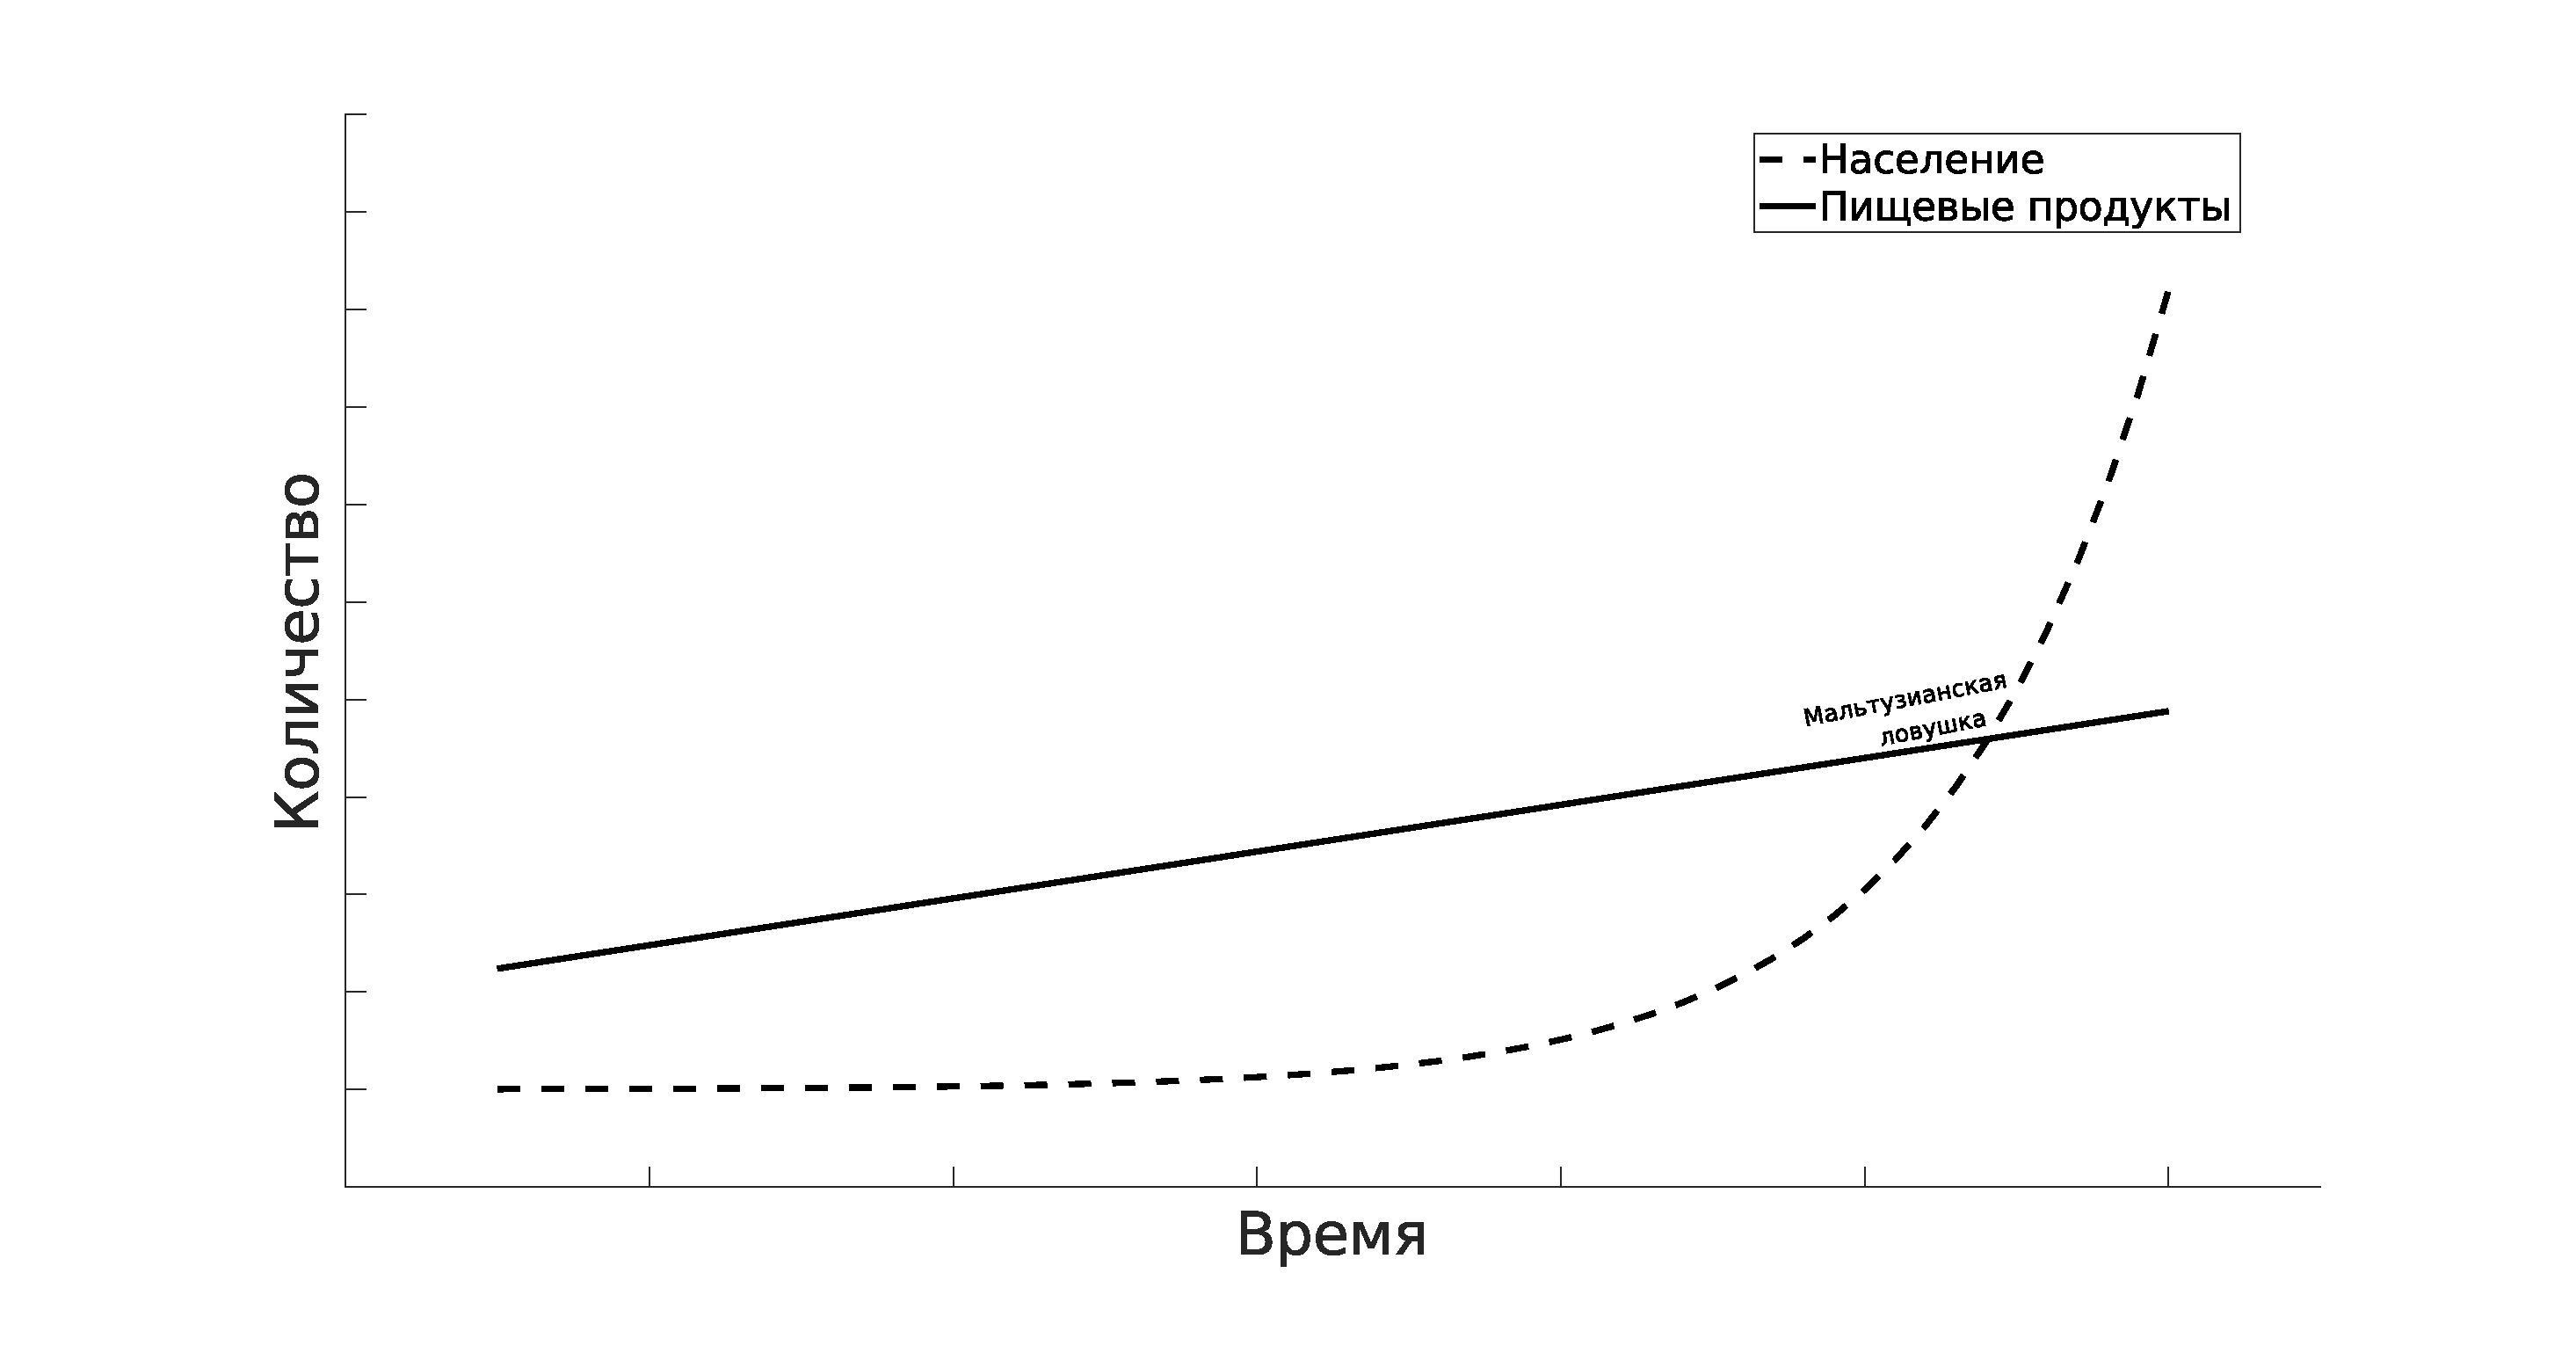
\includegraphics[width = 1.0\textwidth]{malthus.eps}
}
\caption{Мальтузианская ловушка.}
\label{lr_fig2}
\end{figure}

\begin{equation}
\left\{
\begin{array}{rcl}
\dfrac{dN}{dt} &=& rN \Big(1 - \frac{N}{K}\Big), \\
N(0) &=& N_{0}, \quad N_{0} > 0, \\
\end{array}
\right.
\label{lr_eq1}
\end{equation}
где $N(t)$ --- численность популяции, характеризующаяся предельной величиной $K > 0$, которая может быть обеспечена пищевыми ресурсами экологической ниши, в которой обитает вид, а $r > 0$ --- скорость роста. Если численность популяции $N(t)$ мала по сравнению с параметром $K$, мы получаем приближенное уравнение
$$
\frac{dN}{dt} \approx rN,
$$
которое имеет решение $N(t) = N_{0}e^{rt}$. Чтобы получить точное аналитическое решение исходной задачи \eqref{lr_eq1}, нужно первое уравнение системы разделить на $N^{2}$, приняв $n = \frac{1}{N}$. В результате мы получим, что
$$
\frac{dn}{dt} = -rn + \frac{r}{K}.
$$
Сделав еще одну замену, $p = n - \frac{1}{K}$, получим
$$
\frac{dp}{dt} = -rp,
$$
решение которой имеет вид $p(t) = p(0)e^{-rt} = \Big(\frac{1}{N_{0}} - \frac{1}{K}\Big)e^{-rt}$. Сделав обратную замену, получим итоговое решение системы \eqref{lr_eq1}

\begin{equation}
N(t) = N_{0} \frac{K}{N_{0} + (K - N_{0})e^{-rt}}.
\label{lr_eq2}
\end{equation}

Из выражения \eqref{lr_eq2} видно, что в начале происходит экспоненциальный рост популяции, после чего численность стабилизируется и остается на заданном уровне $K$. Кроме того, Ферхюльст показал, что в точке $\frac{K}{2}$ происходит изменение кривизны графика численности популяции с выпуклого на вогнутый, то есть кривая $N(t)$ имеет S - образную форму. Для доказательства данного факта, достаточно рассмотреть знак второй производной $\frac{d^{2}N}{dt^{2}} = r\Big(1 - \frac{2N}{K}\Big)\frac{dN}{dt}$. В силу того, что знак выражения $\frac{dN}{dt}$ всегда больше нуля, имеем, что $\frac{d^{2}N}{dt^{2}} > 0$, если $N < \frac{K}{2}$ и $\frac{d^{2}N}{dt^{2}} < 0$, если $N > \frac{K}{2}$.

Обобщим результаты, полученные Ферхюльстом для случая нескольких видов. Пусть $N_{i}(t)$ --- численность популяции $i$-го вида в момент времени $t$. Согласно закону Мальтуса:
$$
\left\{
\begin{array}{rcl}
\dot{N}_{i}(t) &=& k_{i}N_{i}(t), \quad i = \overline{1, n}\\
N_{i}(0) &=& N_{i}^{0},\\
\end{array}
\right.
$$
где $k_{i}$ --- скорость роста.

Обозначим за $u_{i}(t)$ относительную частоту $i$-го вида

\begin{equation}
u_{i}(t) = \frac{N_{i}(t)}{\sum\limits_{k = 1}^{n}N_{k}(t)},
\label{lr_eq3}
\end{equation}
тогда
$$
\dot{u}_{i}(t) = \frac{\dot{N}_{i}(t)\sum\limits_{k = 1}^{n}N_{k}(t) - N_{i}(t)\sum\limits_{k = 1}^{n}\dot{N}_{k}(t)}{\Big(\sum\limits_{k = 1}^{n}N_{k}(t)\Big)^{2}} = u_{i}(t)(k_{i} - f(t)).
$$

Добавив условие принадлежности относительных частот видов единичному симплексу, получим следующую систему:

\begin{equation}
\left\{
\begin{array}{rcl}
\dot{u}_{i}(t) &=& u_{i}(t)(k_{i} - f(t)), \quad \forall i = \overline{1, n},\\
\sum\limits_{i = 1}^{n} u_{i} &=& 1, \quad u_{i} \ge 0 \quad \forall i = \overline{1, n}.\\
\end{array}
\right.
\label{lr_eq4}
\end{equation}

Данная модель получила название модели ``независимой репликации''\, а величина  
$$
f(t) = \sum\limits_{i = 1}^{n}k_{i}u_{i}(t)
$$ 
--- средний фитнес(приспособленность) системы.

Модель ``независимой репликации''\, является частным случаем репликаторной системы \eqref{intr_eq5} и характеризуется эгоистическим поведением.

Перейдем к исследованию поведения системы \eqref{lr_eq4}. Легко показать, что выживает только тот вид, скорость роста которого максимальна
$$
\dot{\Bigg(\frac{u_{i}}{u_{j}}\Bigg)} = \frac{\dot{u}_{i}u_{j} - u_{i}\dot{u}_{j}}{u_{j}^{2}} = \frac{u_{i}(k_{i} - f)u_{j} - u_{i}u_{j}(k_{j} - f)}{u_{j}^{2}} = \frac{u_{i}}{u_{j}}(k_{i} - k_{j}).
$$
Если $m_{ij} = \dfrac{u_{i}}{u_{j}}$, то получаем $\dot{m}_{ij} = m_{ij}(k_{i} - k_{j})$. Для такой системы существует аналитическое решение
$$
m_{ij} = Ce^{(k_{i} - k_{j})t}.
$$ 
Если $k_{i} = \max(k_{1}, ..., k_{n})$, то при $t \to \infty, m_{ij} \to \infty$, следовательно, в силу ограниченности $u_{j}(t)$, получаем $u_{j}(t) \to 0$.

Рассмотрим подробнее выражение для среднего фитнеса системы $f(t)$. Найдём его производную

\begin{multline*}
\dot{f}(t) = \sum\limits_{i = 1}^{n}k_{i}\dot{u}_{i}(t) = \sum\limits_{i = 1}^{n}k_{i}u_{i}(t)(k_{i} - f(t)) = \sum\limits_{i = 1}^{n}k_{i}^{2}u_{i}(t) - \sum\limits_{i = 1}^{n}k_{i}u_{i}(t)f(t) = \\
= \sum\limits_{i = 1}^{n}k_{i}^{2}u_{i}(t) - \Big(\sum\limits_{i = 1}^{n}k_{i}u_{i}(t)\Big)^{2}.
\end{multline*} 
Теперь вспомним, что такое математическое ожидание и дисперсия некоторой дискретной случайной величины $\xi$:

$$
\mathbb{E}\xi = \sum\limits_{i = 1}^{n}p_{i}\xi_{i},
$$

$$
\mathbb{D}\xi = \mathbb{E}\Big(\xi - \mathbb{E}\xi\Big)^{2} = \mathbb{E}\xi^{2} - \Big(\mathbb{E}\xi\Big)^{2} = \sum\limits_{i = 1}^{n}\xi_{i}^{2}p_{i} - \Big(\sum\limits_{i = 1}^{n}\xi_{i}p_{i}\Big)^{2},
$$
где $p_{i} \in (0, 1)$ и $\sum\limits_{i = 1}^{n}p_{i} = 1$. 

Учитывая, что $\mathbf{u} = (u_{1}, ..., u_{n}) \in S_{n} = \{u_{i}: u_{i} \geqslant 0, \sum\limits_{i = 1}^{n}u_{i} = 1\}$, получаем, что $\dot{f}(t)$ --- это дисперсия, а следовательно, средний фитнес системы не убывает.

В 1930 году была опубликована работа английского ученого Рональда Фишера \cite{Fisher}, в которой была сформулирована теорема, начиная с появления которой, эволюционисты начали применять экстремальные принципы к дарвинской эволюции \cite{Parker}, \cite{grafen1}, \cite{grafen2}. Теорема Фишера утверждает, что интенсивность отбора (и, следовательно, скорость эволюции путем отбора) пропорциональна величине генетической дисперсии по приспособленности эволюционирующей популяции, которая, в свою очередь, пропорциональна эффективному размеру популяции. В дальнейшем данная теорема получила название ``фундаментальной теоремы естественного отбора''\,. 

В оригинале формулировка теоремы звучит следующим образом:\\

\textit{``The rate of increase in fitness of any organism at any time is equal to its genetic variance in fitness at the time.''\,}\\

Следует отметить, что Фишер прямо не конкретизировал понятие \textit{``genetic variance in fitness''\,}. Позднее С.~Райтом было введено другое важное понятие --- адаптация ландшафта приспособленности \cite{wright}. С точки зрения теоретической биологии, ландшафт приспособленности представляет собой гиперповерхноть с холмами, каньонами и долинами. Многие экстремальные принципы эволюции основываются на предположении о том, что эта гиперповерхность статична, а средний фитнес (приспособленность) системы постоянно растет. Таким образом, эволюционный процесс может быть изображен как путь, проходящий через пространство вершин и впадин и заканчивающийся на одном из пиков.

В случае репликаторных систем вполне естественно в качестве ``genetic variance in fitness''\, рассматривать средний фитнес системы. Однако, важно отметить, что в данном случае основная теорема Фишера справедлива когда матрица, описывающая взаимодействие видов, будет симметричной, то есть лишь в случае диплоидной популяции, и совпадение максимального значения средней приспособленности с предельным положением равновесия в системе общего вида является скорее исключением из общего правила чем реальностью \cite{BratusA}. В настоящее время существует множество работ, посвященных новым интерпретациям постулатов Фишера \cite{ewens}, \cite{lessard}, \cite{ao1}, \cite{ao2}. В работе \cite{ao1}, например, новая интерпретация теоремы Фишера о естественном отборе дается в терминах F-теоремы.

Связи процесса биологического естественного отбора и процесса максимизации среднего фитнеса посвящена работа \cite{Brich}, в которой рассматриваются следующие сценарии: система монотонно увеличивает средний фитнес, прекращая изменение при достижении максимума, либо игнорирует временные снижения фитнеса, чтобы в итоге достичь максимального значения. Система \eqref{lr_eq4} относится к системам, для которых реализуется первый вид сценария.

Обобщением системы \eqref{lr_eq4} стала модель, предложенная Манфредом Эйгеном \cite{Eig1} в 1971 году и получившая название системы квазивидов. В дальнейшем эта модель была развита в работах (\cite{Eig2}, \cite{Eig3}). Два основных понятия, рассмотренные авторами в работе --- квазивид и порог ошибок. Эйген описывал квазивид как облако мутантов вокруг наиболее приспособленного генотипа. Математически квазивид --- это собственный вектор эволюционной матрицы (что такое эволюционная матрица будет сказано позже), который соответствует максимальному действительному положительному собственному значению, которое равно средней приспособленности. Существование такого собственного значения является следствием теоремы Фробениуса --- Перрона. Общепринятого определения порога ошибки не существует. Данное понятие было сформулировано с помощью численных вычислений и довольно ошеломляющих цифр \cite{Shuster1}, где не требуется никакого определения, чтобы увидеть порог ошибки в цифрах.  

Для начала рассмотрим подробнее систему в дискретном времени. Она описывает процесс эволюции молекулы ДНК(РНК), представленной в виде нуклеотидной цепочки $\sigma_{i}$ фиксированной длины $L$ и состоящей из нулей и единиц. Очевидно, что общее количество цепочек, которые можно представить таким образом, равно $n = 2^{L}$: 
$$
\sigma_{i} = [a_{0}, a_{1}, ..., a_{L - 1}], \quad i = \overline{0, n - 1}.
$$
Не ограничивая общности, можем считать, что
$$
\sigma_{i} = [a_{0}, a_{1}, ..., a_{L - 1}] \Leftrightarrow i = a_{0} + 2a_{1} + ... + 2^{L - 1}a_{L - 1}, \quad i = \overline{0, n - 1}.
$$  
Обозначим через $N_{i}(t) = N(\sigma_{i}, t)$ --- численность цепочек $i$-го вида в момент времени $t$ и пусть $\sigma_{i}$ порождает, в среднем, $m_{i} = m(\sigma_{i})$ потомков. Через $q_{ij}$ обозначим вероятность того, что при репликации $j$ - го генотипа появится $i$ - ый.

Тогда величина
$$
N_{i}(t + 1) = \sum\limits_{j = 0}^{n - 1}q_{ij}m_{j}N_{j}(t), \quad i = \overline{0, n - 1},
$$
описывает количество цепочек $i$-го типа в момент времени $t + 1$. Если перейти к относительным частотам $u_{i}(t)$ по формуле \eqref{lr_eq3}, получим систему Эйгена в дискретном времени

\begin{equation}
\left\{
\begin{array}{rcl}
\mathbf{u}(t + 1) & = & \dfrac{\mathbf{QMu}(t)}{\overline{m}(t)},\\
\overline{m}(t) & = & \sum\limits_{i = 0}^{n - 1}m_{i}u_{i},\\
\sum\limits_{i = 0}^{n - 1} u_{i} & = & 1.\\ 
\end{array}
\right.
\label{lr_eq5}
\end{equation}
где $\mathbf{u}(t) = \Big(u_{0}(t), u_{1}(t), ..., u_{n - 1}(t)\Big)^{T}$ --- вектор относительных частот, $\mathbf{M} = diag(m_{0}, ..., m_{n - 1})$ --- диагональная матрица, описывающая приспособленность генотипов (также ее еще называют ландшафтом приспособленности), $\overline{m}(t)$ --- средний фитнесс системы, $\mathbf{Q} = [q_{ij}]_{i, j = 0}^{n - 1}$ --- матрица мутаций, которая является стохастической, то есть $\sum\limits_{i = 0}^{n - 1}q_{ij} = 1, \forall j = \overline{0, n - 1}$.

Матрицу $\mathbf{Q}_{m}= \mathbf{QM}$ назовем эволюционной матрицей Эйгена.

Эйген делал предположение, что вероятность мутации $q_{ij}$ зависит только от одного параметра $p \in (0, 1)$ и определяется соотношением
$$
q_{ij} = p^{L - d_{ij}}(1 - p)^{d_{ij}}, \quad i,j = \overline{0, n - 1}
$$
где $d_{ij}$ --- расстояние Хемминга между последовательностями $\sigma_{i}$ и $\sigma_{j}$, то есть число мутаций, необходимых для преобразования $j$-ой цепочки в $i$-ую.

Элементы $q_{ii}$ задают вероятности безошибочного копирования и определяются как
$$
q_{ii} = p^{L}, \quad i = \overline{0, n - 1}.
$$

В непрерывном времени система \eqref{lr_eq5} примет вид

\begin{equation}
\left\{
\begin{array}{rcl}
\dot{u}_{i}(t) & = & \Big(\mathbf{Q}_{m}\mathbf{u}(t)\Big)_{i} - u_{i}(t)f(t), \qquad i = \overline{0, n - 1}\\
f(t) & = & \sum\limits_{i = 0}^{n - 1} m_{i}u_{i},\\
\sum\limits_{i = 0}^{n - 1} u_{i} & = & 1,\\ 
\end{array}
\right.
\label{lr_eq6}
\end{equation}
где $f(t)$ --- средний фитнес системы.

Перейдём к исследованию неподвижной точки системы \eqref{lr_eq6}. Покажем, что она определяется решением задачи на собственные числа для матрицы $\mathbf{Q}_{m}$: $\mathbf{Q}_{m}\overline{\mathbf{u}} = \lambda\overline{\mathbf{u}}$. Умножим обе части равенства на единичный вектор $\mathbf{I} = (1, 1, ..., 1)$.
$$
\Bigg(\mathbf{Q}_{m}\overline{\mathbf{u}}, \mathbf{I}\Bigg) = \sum\limits_{i, j = 0}^{n - 1}q_{ij}m_{j}u_{j} = \sum\limits_{i = 0}^{n - 1}m_{i}u_{i} = \overline{f},
$$

$$
\Big(\lambda\overline{\mathbf{u}}, \mathbf{I}\Big) = \lambda\Big(\overline{\mathbf{u}}, \mathbf{I}\Big) = \lambda\sum\limits_{i = 0}^{n - 1}u_{i} = \lambda.
$$
Таким образом, имеем $\mathbf{Q}_{m}\overline{\mathbf{u}} = \overline{\mathbf{u}}\overline{f}$.

Воспользовавшись теоремой Фробениуса - Перрона мы получим, что для системы Эйгена существует значение $\overline{f}(t)$, которому соответствует неотрицательный вектор $\overline{\mathbf{u}} = (u_{0}, ..., u_{n - 1}) \ge 0$, то есть в данном случае выживают уже несколько видов, а не один как это было для системы \eqref{lr_eq4}. 

Еще один подход перехода от задачи в дискретном виде к непрерывному аналогу --- это предположить, что процессы селекции и мутации независимы. В этом случае мы получим модель Кроу - Кимуры \cite{Crow}, которая имеет следующий вид

\begin{equation}
\left\{
\begin{array}{rcl}
\dot{u}_{i}(t) & = & \Big((\mathbf{M} + \mu \mathbf{Q})\mathbf{u}\Big)_{i} - u_{i}(t)f(t), \qquad i = \overline{0, n - 1}\\
f(t) & = & \sum\limits_{i = 0}^{n - 1} m_{i}u_{i},\\
\sum\limits_{i = 0}^{n - 1} u_{i} & = & 1,\\ 
\end{array}
\right.
\label{lr_eq7}
\end{equation}
где $\mu$ --- скорость мутации. 

В отличие от модели Эйгена, здесь было выдвинуто два значимых предположения, определяющих вид матрицы $\mathbf{Q}$. Во-первых, предполагалось, что число мутаций при переходе от $j$-го генотипа к $i$-му не превышает единицы. Иначе говоря, мы получаем, что $d_{ij} = 1$ когда мутация происходит и $d_{ij} = 0$ в случае безошибочного копирования. При  этом скорость мутации $\mu$ удовлетворяет следующему соотношению:
$$
\left\{
\begin{array}{rcl}
\mu &=& \mu_{0}, \quad \text{если } d_{ij} = 1,\\
\mu &=& -L\mu_{0}, \quad \text{если } d_{ij} = 0,\\
\mu &=& 0, \quad \text{иначе}\\
\end{array}
\right.
$$  
Во-вторых, дабы решить основную проблему, возникающую при моделировании системы \eqref{lr_eq6} --- громоздкость вычислений при достаточно больших $L$,  предполагалось, что цепочки имеющие одинаковое количество единиц в своей записи схлопываются в одну. Это позволяет сократить количество уравнений в системе \eqref{lr_eq7} с $n = 2^{L}$ до $n = L + 1$.

Тогда если $\tilde{\mathbf{Q}}$ --- это матрица мутаций, полученная в результате первого предположения, новая матрица мутаций $\mathbf{Q}$ будет определяться следующим образом:

\begin{equation}
q_{ij} = \dfrac {\sum\limits_{k \in {I}_{i}, s \in {I}_{j}}\tilde{q}_{ks}}{|I_{j}|},
\label{lr_eq8}
\end{equation}  
где $I_{i}$ --- это множество всех цепочек, схлопнувшихся в цепочку $i$.

Рассмотрим данный процесс подробнее при $L = 3$. В этом случае, изначальное число цепочек $n = 2^{L} = 8$:

$
\qquad \qquad \sigma{1} = (0, 0, 0), \quad \sigma{2} = (0, 0, 1), \quad \sigma{3} = (0, 1, 0), \quad \sigma{4} = (0, 1, 1),
$

$
\qquad \qquad  \sigma{5} = (1, 0, 0), \quad \sigma{6} = (1, 0, 1), \quad \sigma{7} = (1, 1, 0), \quad \sigma{8} = (1, 1, 1),
$

и матрица $\tilde{\mathbf{Q}}$ имеет вид

$$
\mathbf{\tilde{Q}} = 
\begin{pmatrix}
-3 & 1 & 1 & 0 & 1 & 0 & 0 & 0\\
1 & -3 & 0 & 1 & 0 & 1 & 0 & 0\\
1 & 0 & -3 & 1 & 0 & 0 & 1 & 0\\
0 & 1 & 1 & -3 & 0 & 0 & 0 & 1\\
1 & 0 & 0 & 0 & -3 & 1 & 1 & 0\\
0 & 1 & 0 & 0 & 1 & -3 & 0 & 1\\
0 & 0 & 1 & 0 & 1 & 0 & -3 & 1\\
0 & 0 & 0 & 1 & 0 & 1 & 1 & -3\\
\end{pmatrix}
$$

После схлопывания число цепочек уменьшается до $n = L + 1 = 4$:

$
\qquad \qquad \underbrace{\sigma{1} = (0, 0, 0)}_{\xi_{1}}, 
\quad \underbrace{\sigma{2} = (0, 0, 1), \quad \sigma{3} = (0, 1, 0)}_{\xi_{2}}, 
\quad \underbrace{\sigma{4} = (0, 1, 1)}_{\xi_{3}},
$

$
\qquad \qquad  \underbrace{\sigma{5} = (1, 0, 0)}_{\xi_{2}}, 
\quad \underbrace{\sigma{6} = (1, 0, 1), \quad \sigma{7} = (1, 1, 0)}_{\xi_{3}}, 
\quad \underbrace{\sigma{8} = (1, 1, 1)}_{\xi_{4}},
$
а множества ${I}_{i}$ имеют вид:

$$
I_{1} = \{1\}, \quad 
I_{2} = \{2, 3, 5\}, \quad 
I_{3} = \{4, 6, 7\}, \quad 
I_{4} = \{8\}.
$$

Тогда, воспользовавшись формулой \eqref{lr_eq8}, мы получим итоговый вид матрицы мутаций $\mathbf{Q}$:

$$
\mathbf{Q} = 
\begin{pmatrix}
-3 & 1 & 0 & 0\\
 3 & -3 & 2 & 0\\
 0 & 2 & -3 & 3\\
 0 & 0 & 1  & -3\\
\end{pmatrix}
$$
Таким образом, общий вид матрицы $\mathbf{Q}$, которую авторы рассматривали в своей работе следующий:

$$
\mathbf{Q} = 
\begin{pmatrix}
-L  & 1     & 0      & 0   & ... & ... & 0\\
L   & -L    & 2      & 0   & ... & ... & 0\\
0   & L - 1 & -L     & 3   & ... & ... & 0\\
0   & 0     & L - 2  & -L  & ... & ... & 0\\
... & ...   & ...    & ... & ... & ... & 0\\
0   & 0     & ...    & ... & 2   & -L  & L\\
0   & 0     & ...    & ... & 0   & 1   & -L\\
\end{pmatrix}
$$

В настоящее время сущетсвует множество работ, посвященных исследованию систем \eqref{lr_eq5}, \eqref{lr_eq6} и \eqref{lr_eq7}. Например, в работах (\cite{Leuth1}, \cite{Leuth2}, \cite{Baake}) показано, что модели Эйгена и Кроу-Кимуры эквивалентны моделям Изинга, что позволяет применять для их исследования методы статистической физики. В работах (\cite{Rumschitzki}, \cite{Garcia}, \cite{Bratus1}) изучаются спектральные свойства эволюционной матрицы Эйгена, а также качественное поведение средней приспособленности системы. В статьях (\cite{Rumschitzki}, \cite{Galluccio}) исследуется решение системы квазивидов, а в статье \cite{Bratus2} приводится его строгий вывод с оценкой скорости сходимости.  

Следующим важным шагом в развитии теории биологической эволюции стало появление работ Эйгена и Шустера (\cite{Eig4}, \cite{Eig5}, \cite{Shuster2}), в которых они рассмотрели модель эволюции гиперциклической репликаторной системы.

Перед тем, как перейти к описанию данной модели, рассмотрим общее репликаторное уравнение, которое моделирует широкий спектр различных биологических явлений, возникающих в совершенно разных эволюционных контекстах (\cite{Hofbauer1}, \cite{Hofbauer2}, \cite{Shuster3}). В частности, это уравнение используется в областях теоретической популяционной генетики (\cite{Hofbauer1}, \cite{Svirezhev}), предбиологической молекулярной эволюции (\cite{Bratus3}, \cite{Bratus4}, \cite{Eig4}, \cite{Eig5}) и эволюционной теории игр (\cite{Hofbauer2}, \cite{Maynard}, \cite{Taylor}).

Чтобы получить общее репликаторное уравнение, рассмотрим следующую систему:

\begin{equation}
\dot{N}_{i}(t) = \Big(\mathbf{AN}(t)\Big)_{i}N_{i}(t), \quad i = \overline{1, n},
\label{lr_eq9}
\end{equation} 
где $N_{i}$ --- абсолютная численность $i$-го вида в момент времени $t$, $\mathbf{A}$ --- матрица взаимодействия.

Перейдем формуле \eqref{lr_eq3} к относительным частотам:

\begin{multline*}
\dot{u}_{i} = \frac{\dot{N}_{i}\sum\limits_{j = 1}^{n}N_{j} - N_{i}\sum\limits_{j = 1}^{n}\dot{N}_{j}}{\Big(\sum\limits_{j = 1}^{n}N_{j}\Big)^{2}} = \sum\limits_{j = 1}^{n}N_{j}\Bigg(\frac{\dot{N}_{i}}{\Big(\sum\limits_{j = 1}^{n}N_{j}\Big)^{2}} - \frac{N_{i}\sum\limits_{j = 1}^{n}\dot{N}_{j}}{\Big(\sum\limits_{j = 1}^{n}N_{j}\Big)^{3}}\Bigg) = \\ 
= \sum\limits_{j = 1}^{n}N_{j}\Bigg(\frac{\Big(\mathbf{AN}\Big)_{i}N_{i}}{\Big(\sum\limits_{j = 1}^{n}N_{j}\Big)^{2}} - u_{i}\frac{\sum\limits_{j = 1}^{1}\Big(\mathbf{AN}\Big)_{j}N_{j}}{\Big(\sum\limits_{j = 1}^{n}N_{j}\Big)^{2}}\Bigg) = \sum\limits_{j = 1}^{n}N_{j}u_{i}\Bigg(\Big(\mathbf{Au}\Big)_{i} - f\Bigg).
\end{multline*} 

В силу того, что

$$
\sum\limits_{j = 1}^{n}N_{j} \ge 0,
$$
полученная система будет топологически орбитально эквивалентна системе \cite{Arnold}

\begin{equation}
\dot{u}_{i}(t) = u_{i}(t)\Bigg(\Big(\mathbf{Au}(t)\Big)_{i} - f(t)\Bigg), \quad i = \overline{1, n}.
\label{lr_eq10}
\end{equation}

Это и есть общее репликаторное уравнение. Величина $f(t)$ --- это средняя приспособленность (фитнес) системы, которая определяется как 
$$
f = \Big(\mathbf{Au, u}\Big) = \sum\limits_{i,j = 1}^{n}a_{ij}u_{i}u_{j}.
$$
Относительные частоты $u_{i}(t)$ удовлетворяют условию 
$$
\sum\limits_{i = 1}^{n} u_{i} = 1.
$$ 
Следовательно, пространство состояний системы \eqref{lr_eq10} --- единичный симплекс
$$
S_{n} = \Bigg\{u_{i}: \sum\limits_{i = 1}^{n} u_{i} = 1, u_{i} \ge 0 \Bigg\},
$$    

Система \eqref{lr_eq10} хорошо изучена в работах (\cite{Eig4}, \cite{Eig5}, \cite{Cressman}). Неподвижная точка данной системы определяется решением системы линейных уравнений

\begin{equation}
\left\{
\begin{array}{rcl}
\Big(\mathbf{Au}\Big)_{1} & = & f\\
\Big(\mathbf{Au}\Big)_{2} & = & f\\
. \quad & . & \quad .\\
\Big(\mathbf{Au}\Big)_{n} & = & f\\
\end{array}
\right.
\label{lr_eq11}
\end{equation}

В общем случае, система \eqref{lr_eq11} может не иметь решения, иметь одно или бесконечно много решений. Необходимое условие существования решения --- линейная зависимость строк матрицы $\mathbf{A}$, то есть существование такого вектора $\alpha \neq 0$:
$$
\sum\limits_{j = 1}^{n}a_{ij}\alpha_{j} = 0, \quad i = \overline{1, n}.
$$ 

В статьях  (\cite{Hofbauer1}, \cite{Hofbauer2}) устанавливается связь между поведением решений репликаторной системы \eqref{lr_eq10} с матрицей взаимодействия $\mathbf{A}$ и одним из основных понятий теории игр --- равновесием по Нэшу с матрицей выишрыша $\mathbf{A}$. 

Напомним, что $\overline{\mathbf{u}} \in S_{n}$ --- положение равновесия по Нэшу, если
$$
\Big(\mathbf{u, A\overline{u}}\Big) \le \Big(\mathbf{\overline{u}, A\overline{u}}\Big), \quad \forall \mathbf{u} \in S_{n}
$$    

Можно показать, что если $\overline{\mathbf{u}}$ --- равновесие по Нэшу игры с матрицей выиграша $\mathbf{A}$, то $\overline{\mathbf{u}}$ --- положение равновесия системы \eqref{lr_eq10} и наоборот, если $\overline{\mathbf{u}}$ --- положение равновесия системы \eqref{lr_eq10} и, кроме того, $\overline{\mathbf{u}}$ устойчиво по Ляпунову, то $\overline{\mathbf{u}}$ --- равновесие по Нэшу.

Одним из примеров репликаторных систем являются гиперциклические репликаторные системы (рис. \ref{lr_fig3}).

\begin{figure}[ht]
\centerfloat{
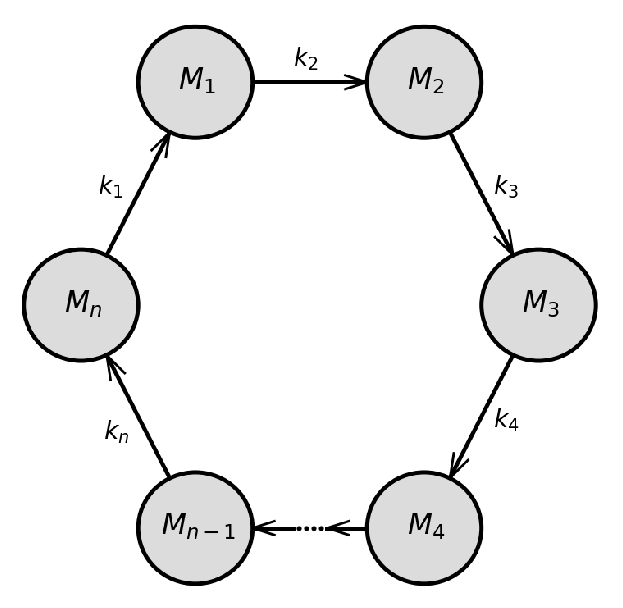
\includegraphics[width = 0.6\linewidth]{hypercycle.eps}
}
\caption{Граф, описывающий гиперциклическую репликацию.}
\label{lr_fig3}
\end{figure}

Модель гиперциклической репликации возникала из попытки ответить на следующий вопрос:\\
 
\textit{``Почему существуют миллионы видов животных и растений, несмотря на то, что молекулярный аппарат клетки в своей основе одинаков: один универсальный код и макромолекулы определенной структуры?''\,}\\

Для объяснения этого факта Эйгеном и Шустером была выдвинута гипотеза о существовании предбиологической эволюции в результате которой могла появится эта универсальная макромолекула, которая предшествовала эволюции всех видов, как макрообъектов биологии. В результате такой эволюции могла возникнуть макромолекула, являющаяся предком макромолекулы РНК. Здесь сразу же возникает вопрос: почему сначала должна была появиться именно макромолекула РНК, а не ДНК или белок? Ответ на этот вопрос дает теория, получившая название гипотезы ``РНК --- мира''\,. Впервые идея ``РНК --- мира''\, была предложена Карлом Везе в 1968 году и развита в дальнейшем Лесли Орджелом и Уолтером Гильбертом. Суть данной теории состоит в том, что для синтеза белков необходима ДНК, копирование же самой ДНК происходит при непосредственном участии белков и РНК. Таким образом, мы получаем диллему ``курицы и яйца''\,. В то же самое время, макромолекула РНК обладает как функциями белков (РНК-катализаторы рибозы), так и функциями ДНК. В настоящее время, теория ``РНК --- мира''\, получила экспериментальное подтверждение.

Уравнение гиперциклической репликаторной системы можно получить из системы \eqref{lr_eq10}, если в качестве матрицы взаимодействия $\mathbf{A}$ рассмотреть матрицу следующего вида:
$$
\mathbf{A} = 
\begin{pmatrix}
0 & 0 & 0 & ... & 0 & 0 & k_{1}\\
k_{2} & 0 & 0 & ... & 0 & 0 & 0\\
0 & k_{3} & 0 & ... & 0 & 0 & 0\\
. & . & . & ... & . & . & .\\
0 & 0 & 0 & ... & k_{n - 1} & 0 & 0\\
0 & 0 & 0 & ... & 0& k_{n} & 0\\
\end{pmatrix}
$$
Тогда система \eqref{lr_eq10} перепишется следующим образом:

\begin{equation}
\left\{
\begin{array}{rcl}
\dot{u}_{i}(t) &=& u_{i}(t)\Big(k_{i}u_{i- 1}(t) - f(t)\Big), \quad i = \overline{1, n},\\
f(t) &=& \sum\limits_{i = 1}^{n}k_{i}u_{i}(t)u_{i - 1}(t)\\
\end{array}
\right.
\label{lr_eq12}
\end{equation}  

Долгая история исследования гиперциклических систем выявила, что они обладают рядом замечательных свойств, присущих биологическим системам, удовлетворяющим дарвинской триаде: наследственность, изменчивость и борьба за существование. Первое из указанных свойств обеспечивается свойством перманентности гиперцикла: при ненулевых начальных данных в процессе динамики ни одна из макромолекул гиперцикла не исчезает. Кроме того, фазовые траектории системы при размерности $n \ge 5$ сходятся к устойчивому предельному циклу. Второе свойство следует из адаптивности гиперцикла, заключающейся в возможности замены одного из элементов гиперцикла любым мутантом, который адаптирован к условиям среды лучше, чем другие элементы системы. В этом случае средняя приспособленность системы может только возрасти. И, наконец, третье свойсто дарвинской триады является следствием того факта, что в динамической системе состоящей из ряда гиперциклов выживает лишь один. 

Все это позволяет рассматривать гиперциклические системы в качестве подходящей математической модели для описания предбиологической эволюции. Однако существует значительное препятствие для распространения данной теории. Это существование так называемых ``паразитов''\, --- макромолекул, которые пользуясь альтруизмом макромолекул гиперцикла получают бесплатное питание за их счет, при этом ничего не отдавая взамен (рис. \ref{lr_fig4}). В итоге, это приводит к полному разрушению системы. 

\begin{figure}[ht]
\centerfloat{
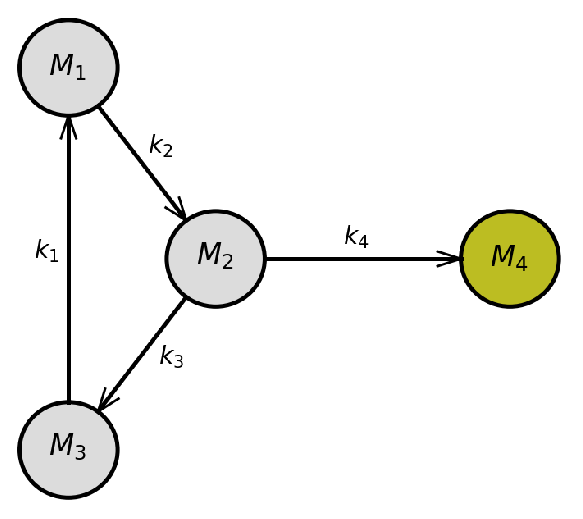
\includegraphics[width = 0.6\linewidth]{parasit_hypercycle.eps}
}
\caption{Граф, описывающий взаимодействие гиперцикла 3-го порядка с паразитом}
\label{lr_fig4}
\end{figure}

Одно из возможных решений проблемы вторжения паразитов было предложено в \cite{Boerlijst} и применено в \cite{Szab}, где гиперциклическая система имела явную пространственную структуру и исследовалась с помощью моделирования клеточных автоматов. Аналогичная идея лежит в основе другой статьи \cite{Bresch} и последующих исследований (\cite{Hogeweg}, \cite{Takeuchi}). Можно обратиться к исследованию \cite{Sigmund}, чтобы узнать подробности о балансе между альтруизмом и эгоистичностью и его влиянии на поведение системы.

Помимо систем обычных гиперциклов, в которых скорость изменения количества (концентрации) макромолекул зависит от количества (концентрации) данной макромолекулы и предыдущей, существуют системы кратных гиперциклов. По своим свойствам они схожи с обычными гиперциклами: например, так же удовлетворяют триаде Дарвина или погибают под воздействием паразитов. Но теперь каждая макромолекула катализируется с помощью нескольких предыдущих. Рассмотрим, например, систему двойного гиперцикла (бигиперцикла)

\begin{equation}
\dot{u}_{i}(t) = u_{i}(t)\Big(k_{i}k_{i - 1}u_{i- 1}(t)u_{i - 2}(t) - f(t)\Big), \quad i = \overline{1, n},
\label{lr_eq13}
\end{equation}  
где $k_{0} = k_{n}, u_{0}(t) = u_{n}(t), u_{-1}(t) = u_{n - 1}(t)$. 

Уравнение \eqref{lr_eq13} может быть получено из уравнения
$$
\dot{N}_{i}(t) = k_{i}k_{i - 1}N_{i}(t)N_{i - 1}(t)N_{i - 2}(t), \quad i = \overline{1, n},
$$
с помощью перехода к относительным частотам по формуле \eqref{lr_eq3}, аналогично тому, как это делалось для системы \eqref{lr_eq10}.

\begin{figure}[ht]
\centerfloat{
\includegraphics[width = 0.6\linewidth]{behypercycle.eps}
}
\caption{Граф, описывающий бигиперциклическую систему $n$-го порядка}
\label{lr_fig5}
\end{figure}

Средний фитнес такой системы определяется следующим образом
$$
f(t) = \sum\limits_{i = 1}^{n}k_{i}k_{i - 1}u_{i}(t)u_{i - 1}(t)u_{i - 2}(t).
$$

Из уравнения \eqref{lr_eq13} видно, что репликация каждого вида происходит с помощью двух предыдущих в замкнутом цикле. Граф взаимодействия для системы бигиперцикла представлен на рис. \ref{lr_fig5}.

Следует отметить, что идеи М. Эйгена получают практическое подтверждение. Так, например, в работе \cite{Lincoln} построен гиперцикл, состоящий из двух макромолекул, а в работе \cite{Vaidya} рассмотрены биохимические реакции системы гиперцикла шестого порядка.



